\documentclass[a4paper,11pt]{article}

%%
%% WCCM Template
\usepackage[ left   = 25.4mm
           , right  = 25.4mm
           , top    = 25.4mm
           , bottom = 25.4mm
           ]{geometry}
\usepackage{authblk}
\usepackage[T1]{fontenc}
\usepackage{graphicx}
\usepackage{nopageno}
\usepackage{parskip}
\usepackage{titlesec}
\usepackage{etoolbox}
\usepackage{soul}
\usepackage[hidelinks]{hyperref}
\usepackage{siunitx}
\usepackage{amsmath}
\usepackage{amssymb}
\usepackage{amsfonts}
\usepackage[capitalise,noabbrev,nameinlink]{cleveref}
\usepackage[nolist,nohyperlinks]{acronym}
\usepackage{times}
\usepackage[numbers,sort&compress]{natbib}
\usepackage{etoolbox}
\usepackage{ifthen}
\usepackage[font=small]{caption}
\usepackage{subcaption}
\usepackage{setspace}

%%
%% Custom SI Units
\DeclareSIUnit\point{\ensuremath{\mathrm{pt}}}

%%
%% Author Block

%% Corresponding author commands
\newlength{\corsep}\setlength{\corsep}{18pt}
\newcommand{\corfont}{\itshape}
\newcommand{\corsymb}{\textsuperscript{\textdagger}}
\newcommand{\corauth}[1]{\author[ ]{#1\corsymb}}

%% Title Block
\makeatletter
\newcommand{\email}[1]{\edef\@email{#1}}
\newcommand{\coraffil}[1]{\edef\@coraffil{#1}}

\renewcommand{\maketitle}{%
\begin{center}
    {\normalfont\noindent\ignorespaces\bfseries\@title\par}
    \vspace{-7.0pt}
    {\linespread{1.75}\noindent\ignorespaces\@author\par}

\end{center}}

\renewcommand{\Affilfont}{\normalsize}
\renewcommand\@author{%
  \ifx\AB@affillist\AB@empty%
    \AB@author%
  \else
    \ifnum\value{affil}>\value{Maxaffil}%
      \def\rlap##1{##1}%
      \AB@authlist\\[0.5\corsep]%
        {{\normalfont\corsymb}\corfont\@coraffil\\[-5pt]{\normalfont\corsymb}E-mail: \href{mailto:\@email}{\@email}}\\[0.25\affilsep]%
        \AB@affillist
    \else%
      \AB@authors%
    \fi%
  \fi}
\makeatother

%% Settings
\renewcommand*{\Authsep}{, }
\renewcommand*{\Authand}{, }
\renewcommand*{\Authands}{and }
\renewcommand*{\Authfont}{\normalfont\footnotesize}
\renewcommand*{\Affilfont}{\itshape\footnotesize}
\setlength{\affilsep}{12pt}

%%
%% Abstract
\makeatletter
\renewenvironment{abstract}{%
  \renewcommand{\baselinestretch}{1.0} 
  \vspace*{5mm}
  \noindent\begin{minipage}{1\textwidth}
  \textbf{Abstract}\bigskip

  %\normalfont\small\selectfont
  \normalfont\normalsize\selectfont
  \medskip

}{\end{minipage}}
\makeatother

%%
%% Keywords
\makeatletter
\newenvironment{keywords}{%
  \renewcommand{\baselinestretch}{1.0} 
  \medskip\noindent\begin{minipage}{1\textwidth}\textbf{Keywords:}
}{\end{minipage}\vspace{10pt}}
\makeatother

%%
%% Acknowledgements
\makeatletter
\newenvironment{acknowledgment}{%
    \medskip
    \noindent\begin{minipage}{1\textwidth}
    \section*{Acknowledgments}
}{\end{minipage}}
\makeatother

%%
%% Reformatting Table and Figure lables
%\renewcommand{\tablename}{\small\selectfont Tab.}
%\renewcommand{\figurename}{\small Fig.}
%\setlength\abovecaptionskip{2pt}
\setlength\belowcaptionskip{-7.5pt}

%%
%% Section formatting
\titleformat{\section}{\normalsize\normalfont}{\textbf{\thesection}}{0.5em}{\textbf}
\titleformat{\subsection}{\normalsize\normalfont}{\textbf{\thesubsection}}{0.5em}{\textbf}
\titleformat{\subsubsection}{\normalsize\normalfont}{\textbf{\thesubsubsection}}{0.5em}{\textbf}

\titlespacing{\section}{0pt}{10pt}{10pt}
\titlespacing{\subsection}{0pt}{10pt}{10pt}
\titlespacing{\subsubsection}{0pt}{10pt}{10pt}

%%
%% No paragraph indentation
\setlength{\parindent}{0pt}
\setlength{\parskip}{12pt} 

%%
%% 1.5 × Line Spacing
\makeatletter
\let\@currsize\normalsize
\makeatother
\renewcommand{\baselinestretch}{1.5} 

\acrodef{WCCM}{world congress on condition monitoring}


%%
%% Paper Title
\title {Template for producing a full paper manuscript for submission to the
  3\textsuperscript{rd} World Congress on Condition Monitoring (WCCM2024)}

%%
%% Author Block
\corauth{C. D. FamilyName}
\author[1]{A. B. FamilyName}
\author[2]{E. F. FamilyName}
\coraffil{Department, University/Company Name, Address, City, Country.}
\affil[1]{Department, University/Company Name.}
\affil[2]{Department, University/Company Name.}
\email{cd\_author@company.com}

\begin{document}

%%
%% Header Formatting and Title
\maketitle

%%
%% Use abstract environment for the abstract
\begin{abstract}
The abstract should appear as a single paragraph justified against both
margins. Page size is fixed as A4. Margins set at \qty{25.4}{\milli\meter} /
\qty{2.54}{\centi\meter} / \num{1}~inch at all sides. The font should be set as
Times New Roman throughout. Title should be \qty{11}{\point} bold centred.
Author names should be \qty{9}{\point} regular centred. Author affiliations
should be \qty{9}{\point} italic centred. Full contact details should only be
provided for the corresponding author. Abstract body text should be
\qty{10}{\point} regular, single spaced. Please contact the Conference
Secretariat by email to \href{mailto:3rdwccm@csei.org.cn}{3rdwccm@csei.org.cn}
if you require any clarification on full paper format or submission procedure.
\end{abstract}

%%
%% Use keywords environment for the keywords
\begin{keywords}
Please list a maximum of \num{6} keywords or phrases
\end{keywords}

%%
%% Main body
\section{Section}

Page size is fixed as A4. Margins set at \qty{25.4}{\milli\meter} /
\qty{2.54}{\centi\meter} / \num{1}\,inch at all sides. The font should be set
as Times New Roman throughout. All body text should be justified against both
margins. Body text should be \qty{11}{\point} regular.
Line spacing should be \num{1.5} times. A \qty{12}{\point} space should be left
between each paragraph. Section headings at all levels should be
\qty{11}{\point} bold. Full paper manuscripts should contain
\numrange[range-phrase = --]{6}{8} pages.

\subsection{Sub-Section}

All body text should be justified against both margins. Body text should be
\qty{11}{\point} regular. Line spacing should be \num{1.5} times. A
\qty{12}{\point} space should be left between each paragraph. Section headings
at all levels should be \qty{11}{\point} bold.

\subsubsection{Sub-Sub-Section}

All body text should be justified against both margins. Body text should be
\qty{11}{\point} regular. Line spacing should be \num{1.5} times. A
\qty{12}{\point} space should be left between each paragraph. Section headings
at all levels should be \qty{11}{\point} bold.

\section{Section}

References should be cited in numeric order and enclosed within square brackets
at the end of sentence prior to the full stop~\cite{qi22}.

Figures including drawings, graphs, images and photographs should be inserted
as close as possible to where they are described. All figures must be cited
within the text. Figures should be numbered consecutively. Figures should be
centred within the page margins. No text within any figure should be smaller
than \qty{10}{\point}. All figures should have a descriptive caption placed
below the figure, see \cref{fig:bad} below. 

\begin{figure}[h]
  \centering
  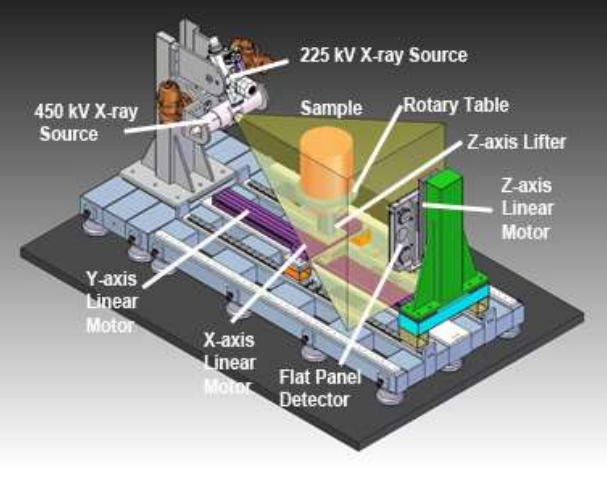
\includegraphics[width=0.75\textwidth]{./fig/bad-fig.png}
  \caption{Captions for figures should be \qty{10}{\point} regular centered.
  }\label{fig:bad}
\end{figure}

All body text should be justified against both margins. Body text should be
\qty{11}{\point} regular. Line spacing should be \num{1.5} times. A
\qty{12}{\point} space should be left between each paragraph. 

\section{Section}

Tables should be inserted as close as possible to where they are described. All
tables must be cited within the text. Tables should be numbered consecutively.
Tables should be centred within the page margins. No text within a table should
be smaller than \qty{10}{\point}. All tables should have a descriptive caption 
placed below the table, see \cref{tab:bad} below. If a table is broken across a
page break, please repeat column headings after the page break.

\begin{table}[h]
  \centering
  \begin{tabular}{| c | c | c |}
    \hline
    Column 1 & Column 2 & Column 4 \\
    \hline
    1 & 2 & 3 \\
    \hline
    2 & 4 & 6 \\
    \hline
  \end{tabular}
  \caption{Descriptive caption for tables should be \qty{10}{\point} centred.
  }\label{tab:bad}
\end{table}

All body text should be justified against both margins. Body text should be
\qty{11}{\point} regular. Line spacing should be \num{1.5} times. A
\qty{12}{\point} space should be left between each paragraph. 

\section{Guidelines}

\subsection{Abbreviations}

Define abbreviations and acronyms the first time they are used. Standard and
well-known abbreviations do not need to be defined. Abbreviations that include
full stops should not have spaces: write ``A.B.C.D'' not ``A. B. C. D.''. 
Please follow the example in \texttt{./acronyms.tex} to use acronyms such as
the \ac{WCCM}.

\subsection{Units}

Please use the \texttt{qty} and \texttt{num} commands from \texttt{siunitx}
package to ensure consistent number and unit formatting. 

\subsection{Equations}

Equations should be numbered consecutively with equation numbers in parentheses
flush with the right margin, as in \eqref{eq:bad}. Symbols used in equations
should be defined before the equation appears or immediately following the
equation. 

\begin{equation}\label{eq:bad}
  f(x) = a_{0} + \sum_{n = 1}^{\infty} \left( a_{n} \cos \frac{n\pi x}{L} + b_{n} \sin \frac{n\pi x}{L}\right)
\end{equation}

Symbols should be italicised. Refer to ``\eqref{eq:bad}'' not
``Eq. \eqref{eq:bad}'' or ``\cref{eq:bad}'' except at the beginning of 
a sentence where ``\Cref{eq:bad} \dots'' should be used. Please ensure that all
text and symbols in an equation are no smaller than \qty{10}{\point}.

\subsection{Other Recommendation}

Use one space after full stops and colons. Hyphenate complex modifiers. Use a
zero before a decimal point: ``\num{0.25}'' not
``\num[print-zero-integer=false]{0.25}''. Leave one protected half space between
a quantity and its unit: ``\qty{1.4}{\watt}'' not ``$1.4\mathrm{W}$''. Prefixes 
such as ``non'', ``sub'', ``micro'' etc., are not independent words; they
should be joined to the words they modify using a hyphen. Avoid hanging lines
across page breaks. 

%%
%% Use acknowledgment environment for the acknowledgments
\begin{acknowledgment}
All body text should be justified against both margins. Body text should be
\qty{11}{\point} regular. Line spacing should be \num{1.5} times. A
\qty{12}{\point} space should be left between each paragraph.
\end{acknowledgment}

%%
%% Bibliography
\begingroup
  \bibliographystyle{IEEEtranS}
  \setstretch{1}
  \bibliography{bibliography}
\endgroup

For two authors please use ``A. B. FamilyName and C. D. FamilyName''. For three
authors please use ``A. B. FamilyName, C. D. FamilyName, and E. F.
FamilyName''. For more than \num{3} authors please use ``A. B. FamilyName and
others'' for the \texttt{author} field in \texttt{./bibliography.bib}. 

\end{document}
